\usepackage{ucll-code}

\usetikzlibrary{shadows,shapes.multipart}

\title{Pointers}
\author{Fr\'ed\'eric Vogels}


\begin{document}

\begin{frame}
  \titlepage
\end{frame}


\begin{frame}
  \frametitle{Argument Passing in Java}
  \code[language=java,font=\small]{pass-int.java}
  \begin{itemize}
    \item Primitive types are passed by value
    \item All of \texttt{x}'s bits are copied to the stack
    \item \texttt{foo} is unable to modify \texttt{x}'s value
  \end{itemize}
\end{frame}

\begin{frame}
  \frametitle{Argument Passing in Java}
  \code[language=java,font=\small]{pass-int-array.java}
  \begin{itemize}
    \item Objects are passed by reference
    \item \texttt{foo} can modify the array
  \end{itemize}
\end{frame}

\begin{frame}
  \frametitle{Why This Inconsistency?}
  \begin{itemize}
    \item Primitives: by value
    \item Objects: by reference
    \item Why not everything the same way?
  \end{itemize}
\end{frame}

\begin{frame}
  \frametitle{Reason \#1: Efficiency}
  \begin{itemize}
    \item Say objects are passed by value
    \item In case of array, all elements would have to be copied
    \item Uses a lot of time and memory
    \item References have constant size: 32 or 64 bit
    \item Fit in register
    \item You can give access to arbitrarily large data structures using a single reference
  \end{itemize}
\end{frame}

\begin{frame}
  \frametitle{Reason \#2: Sharing}
  \begin{itemize}
    \item References allow you to ``share'' objects
    \item If objects were always passed by value, you could not pass the \emph{same} object to two different objects
  \end{itemize}

  \begin{center}
    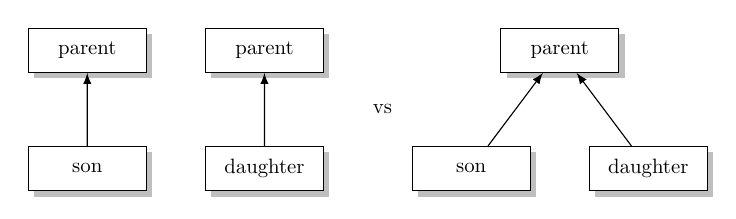
\begin{tikzpicture}[person/.style={fill=white,drop shadow,draw,minimum width=2cm,minimum height=.75cm},scale=.75,transform shape]
      \begin{scope}
        \node[person] (parent1) at (-1.5,2) {parent};
        \node[person] (parent2) at (1.5,2) {parent};
        \node[person] (son) at (-1.5,0) {son};
        \node[person] (daughter) at (1.5,0) {daughter};
        \draw[-latex] (son) -- (parent1);
        \draw[-latex] (daughter) -- (parent2);
      \end{scope}

      \node at (3.5,1) {vs};

      \begin{scope}[xshift=6.5cm]
        \node[person] (parent) at (0,2) {parent};
        \node[person] (son) at (-1.5,0) {son};
        \node[person] (daughter) at (1.5,0) {daughter};
        \draw[-latex] (son) -- (parent);
        \draw[-latex] (daughter) -- (parent);
      \end{scope}
    \end{tikzpicture}
  \end{center}
\end{frame}

\begin{frame}
  \frametitle{Reason \#3: Recursion and \texttt{null}}
  \code[language=java]{person.java}
  \begin{itemize}
    \item Without references, no recursive data structures
    \item \texttt{Person} would be infinitely large
    \item Thanks to references, a \texttt{Person} is only 64/128 bit large
    \item \texttt{null} can be used to end chains
  \end{itemize}
\end{frame}

\begin{frame}
  \frametitle{Reason \#4: Giving Access}
  \code[language=java]{this.java}
  \begin{itemize}
    \item Without references, functions would never be able to modify their arguments
    \item Without references, \texttt{this} would be a copy
    \item Methods would never be able to modify the object's fields
  \end{itemize}
\end{frame}

\begin{frame}
  \frametitle{References in Java}
  \begin{itemize}
    \item Whether \texttt{T x} is a reference, depends on the type \texttt{T}
          \begin{itemize}
            \item If \texttt{T} is primitive, then it's not a reference
            \item If \texttt{T} is a class, then it's a reference
          \end{itemize}
    \item No extra syntax needed to discern references from values
  \end{itemize}
  \begin{center}
    \begin{tabular}{ccc}
        & \textbf{primitive} & \textbf{class} \\
      \toprule
      \textbf{value} & yes & not supported \\
      \textbf{reference} & not supported & yes \\
    \end{tabular}
  \end{center}
\end{frame}

\begin{frame}
  \frametitle{Pointers in \cpp}
  \begin{center}
    \begin{tabular}{ccc}
        & \textbf{primitive} & \textbf{class} \\
      \toprule
      \textbf{value} & yes & yes \\
      \textbf{pointer} & yes & yes \\
    \end{tabular}
  \end{center}
  \begin{itemize}
    \item \cpp\ provides \emph{pointers}
    \item Fulfill same role as references as in Java
    \item \cpp\ do not treat primitives and classes differently
          \begin{itemize}
            \item Java does not allow reference to primitive
            \item \cpp\ allows pointer to primitive
          \end{itemize}
    \item How to know if you want pointer or not?
    \item Extra syntax needed!
    \item Value: \texttt{T x}
    \item Pointer: \texttt{T* x}
  \end{itemize}
\end{frame}

%%% Local Variables:
%%% mode: latex
%%% TeX-master: "pointers"
%%% End:

\begin{frame}
  \frametitle{Pointers}
  \begin{itemize}
    \item Pointers have a reputation
    \item Pointers are \emph{not} hard
    \item If you can work with arrays in Java, you can work with pointers in \cpp
    \item Pointers are \emph{fragile} though
    \item Easy to make mistakes
    \item But that's ok, because they're really simple
  \end{itemize}
\end{frame}

\begin{frame}
  \frametitle{Memory: A Simple Model}
  \begin{itemize}
    \item Memory can be seen as one gigantic {\tt byte[]} array
    \item Every time you need memory (e.g.\ a stack-variable, a heap-object, \dots)
          a little part of this array is given to you
    \item You could assign ranges to the different allocation methods, e.g.
          \begin{itemize}
            \item Static allocation: first 1000000 bytes
            \item Stack: following 1000000 bytes
            \item Heap: all the rest
          \end{itemize}
          but making this distinction not important right now
  \end{itemize}
\end{frame}

\begin{frame}
  \frametitle{Memory as a {\tt byte[]}}
  \begin{center}
    \begin{tikzpicture}[scale=.25,transform shape]
      \only<2->{
        \draw[fill=red!50] (7,0) rectangle ++(4,1);
      }

      \visible<3|handout:1>{
        \foreach \i in {0,...,39} {
          \node[anchor=west,rotate=90] at ($ (\i,1) + (.5,0) $) {
            \tikzmath{
              int \address;
              \address = 4684 + \i;
               print {\tt\address};
            }
          };
        }
      }

      \visible<4-|handout:0>{
        \foreach \i in {0,...,39} {
          \node[anchor=west,rotate=90] at ($ (\i,1) + (.5,0) $) {
            \tikzmath{
              int \address;
              \address = hex(4684 + \i);
               print {\tt0x\address};
            }
          };
        }
      }
      
      \visible<0|handout:1>{
      	\foreach \i in {0,...,39} {
      		\node[anchor=west,rotate=90] at ($ (\i,2.5) + (.5,0) $) {
      			\tikzmath{
      				int \address;
      				\address = hex(4684 + \i);
      				print {\tt0x\address};
      			}
      		};
      	}
      }

      \draw (0,0) grid (40,1);
      \node[anchor=east,font=\Huge] at (0,0) {$\cdots$};
      \node[anchor=west,font=\Huge] at (40,0) {$\cdots$};
    \end{tikzpicture}
  \end{center}
  \begin{itemize}
    \item If you need an {\tt int x} variable somewhere four consecutive bytes will be required to store {\tt x}
    \item<3-> Since memory is a {\tt byte[]}, every byte has a unique index
    \item<4-> We can write this index in hexadecimal
    \item<5-> In the above figure: {\tt x} occupies bytes with indices 
              \begin{center}
                {\tt 0x1253}, {\tt 0x1254}, {\tt 0x1255}, {\tt 0x1256}
              \end{center}
    \item<5-> The index of the first byte of {\tt x} is the \emph{address} of {\tt x}
    \item<5-> Address of {\tt x} is {\tt 0x1253}
  \end{itemize}
\end{frame}

\begin{frame}
  \frametitle{A New Type}
  \begin{itemize}
    \item Say we have a variable {\tt int x}
    \item {\tt x} must have an address
    \item You can ask for this address
    \item New type: ``address of {\tt int}''
  \end{itemize}
  \vskip1cm
  \code[frame=lines,font=\small,language=c++14]{address-of.cpp}
\end{frame}

\begin{frame}
  \frametitle{What Does One Do With An Address?}
  \begin{itemize}
  \item If you know where a variable resides in memory
        (i.e.\ if you have its address), then you can read and write to it
  \end{itemize}
  \vskip1cm
  \code[frame=lines,font=\small,language=c++14]{use-address.cpp}
\end{frame}

\begin{frame}
  \frametitle{Quiz}
  \begin{itemize}
    \item Integer division {\tt x / y} has two results:
          \begin{itemize}
            \item Quotient {\tt q}
            \item Rest {\tt r}
          \end{itemize}
    \item {\tt q * y + r = x}
    \item How to write a function {\tt div} that returns quotient and rest?
  \end{itemize}
\end{frame}

\begin{frame}
  \frametitle{Div in Java: Attempt \#1}
  \code[language=java,font=\small,frame=lines]{div1.java}
  \vskip5mm
  \structure{Evaluation}
  \begin{procontralist}
    \con Need for array creation on heap (slow)
    \con Type \texttt{int[]} does not tell there will be 2 retvals
    \con Compiler does not enforce correct number of retvals
    \con Works only if function returns values of same type
    \con No naming (is {\tt q} the first or second element?)
  \end{procontralist}
\end{frame}

\begin{frame}
  \frametitle{Div in Java: Attempt \#2}
  \code[language=java,font=\small,frame=lines]{div2.java}
  \structure{Evaluation}
  \begin{procontralist}
    \pro Type safe
         \begin{itemize}
           \item \texttt{div} cannot return wrong number of results
           \item All type combinations possible
         \end{itemize}
    \pro Naming of results
    \con Need for object creation on heap (slow)
    \con Lots of ``stupid code'' necessary: we would need to define a new class for each function returning multiple values
  \end{procontralist}
\end{frame}

\begin{frame}
  \frametitle{Div in Java: Attempt \#3}
  \code[language=java,font=\small,frame=lines,width=.9\linewidth]{div3.java}
  \structure{Evaluation}
  \begin{procontralist}
    \pro Type safe
    \pro Reusable {\tt Pair} class
    \con Need for three (!) object creations on heap
    \con No naming
    \con Boilerplate code alert: {\tt Triple}, {\tt Quadruple}, \dots
  \end{procontralist}
\end{frame}

\begin{frame}
  \frametitle{Div in Java: Attempt \#4}
  \code[language=java,font=\small,frame=lines]{div4.java}
  \structure{Evaluation}
  \begin{procontralist}
    \pro Type safe
    \pro No heap allocations necessary
    \pro Clear naming
    \con Ideal, except that it doesn't work \frownie
  \end{procontralist}
\end{frame}

\begin{frame}
  \frametitle{\cpp\ To The Rescue!}
  \code[language=c++14,width=\linewidth]{div.cpp}
\end{frame}

\begin{frame}
  \frametitle{Pass-by-value vs ``Pass-by-address''}
  \begin{itemize}
    \item Passing \texttt{q} and \texttt{r} as regular \texttt{int}s does not work:
          copies are given to \texttt{div} and no matter what \texttt{div} does,
          it has no effect on \texttt{func}'s \texttt{q} and \texttt{r}
    \item Passing the \emph{addresses} of \texttt{q} and \texttt{r} allows \texttt{div} to access \texttt{func}'s local
          variables: it knows where they live!
    \item This technique is called ``out parameters'': using parameters for \emph{output}
  \end{itemize}
\end{frame}

\begin{frame}
  \frametitle{Syntax}
  \structure{Pseudosyntax}
  \code[frame=lines,language=c++14]{pointer-syntax.cpp}
  \vskip5mm
  \structure{\cpp\ syntax}
  \code[frame=lines,width=.4\linewidth,language=c++14]{pointer-syntax2.cpp}

  \begin{tikzpicture}[overlay,remember picture,box/.style={red,thick}]
    \only<2|handout:0>{
      \drawboxaround{address of int}
      \drawboxaround{int pointer}
    }
    \only<3|handout:0>{
      \drawboxaround{address of}
      \drawboxaround{address of operator}
    }
    \only<4|handout:0>{
      \drawboxaround{write to}
      \drawboxaround{write to syntax}
    }
  \end{tikzpicture}
\end{frame}

\begin{frame}
  \frametitle{Syntax}
  \begin{center}
    \begin{tabular}{ll}
      \textbf{Syntax}  & \textbf{Description} \\
      \toprule
      {\it type}*      & Pointer to a {\it type} \\
      \&{\it variable} & Address of {\it variable} \\
      *{\it pointer}   & Dereference pointer \\
    \end{tabular}
  \end{center}
  \begin{itemize}
    \item A \emph{pointer} is a variable that contains an address
    \item To access whatever is located at the address, you \emph{dereference} the pointer
    \item The {\tt \&} and {\tt *} need to be balanced
    \item Similar to arrays: given a {\tt T[] xs} you need to index {\tt xs} to reach a {\tt T}
  \end{itemize}
\end{frame}

%%% Local Variables:
%%% mode: latex
%%% TeX-master: "pointers"
%%% End:

\section{Examples}
\subsection{Indexing}
\frame{\tableofcontents[currentsubsection]}

\begin{frame}
  \frametitle{\tt Indexing}
  \begin{itemize}
    \item Indexing \texttt{[]} only defined on pointers/arrays
    \item However, you can overload \texttt{[]} for your own containers
    \item For example, \texttt{std::vector} overloads \texttt{[]}
  \end{itemize}
  \code[font=\small]{vector.cpp}
\end{frame}

\subsection{\texttt{toString}}
\frame{\tableofcontents[currentsubsection]}

\begin{frame}
  \frametitle{\texttt{toString} in \cpp}
  \code{cout.cpp}
  \begin{itemize}
    \item How to make this work?
  \end{itemize}
\end{frame}

\begin{frame}
  \frametitle{\texttt{toString} in \cpp}
  \code[font=\small,width=.9\linewidth]{cout-sol.cpp}
  \begin{itemize}
    \item Solution: overload \texttt{<<} on \texttt{std::ostream}
  \end{itemize}
\end{frame}

\subsection{Assignment}
\frame{\tableofcontents[currentsubsection]}

\begin{frame}
  \frametitle{Assignment}
  \code{assignment.cpp}
  \begin{itemize}
    \item By default, assignment \emph{between objects} overwrites the fields of the left operand
          with the values of the fields of the right operand
    \item \texttt{x} and \texttt{y} are still distinct objects after assignment
  \end{itemize}
\end{frame}

\begin{frame}
  \frametitle{Assignment}
  \begin{itemize}
    \item Do not confuse with assignment in Java!
    \item Java assignment operates on pointers
  \end{itemize}
  \code[width=.9\linewidth]{assignment-comparison.cpp}
\end{frame}

\begin{frame}
  \frametitle{Assignment}
  \code{intlist-assignment.cpp}
  \begin{itemize}
    \item Default behaviour is not always what we want
    \item \texttt{xs} and \texttt{ys} would share same internal array
    \item We need \texttt{xs} and \texttt{ys} to have separate internal arrays
    \item We need to redefine \texttt{=} on \texttt{IntList}
  \end{itemize}
\end{frame}

\begin{frame}
  \frametitle{Assignment}
  \code[font=\small,width=.9\linewidth]{intlist-assignment-corrected.cpp}
\end{frame}

%%% Local Variables:
%%% mode: latex
%%% TeX-master: "operator-overloading"
%%% End:


\begin{frame}
  \frametitle{Summary}
  \begin{center}
    \begin{tabular}{ll}
      \textbf{Syntax}  & \textbf{Description} \\
      \toprule
      {\it type}*      & Pointer to a {\it type} \\
      \&{\it variable} & Address of {\it variable} \\
      *{\it pointer}   & Dereference pointer \\
    \end{tabular}
  \end{center}
  \structure{Typical Usage}
  \begin{enumerate}
    \item Introduce some variable \texttt{x} of type \texttt{T}
    \item Take the address of \texttt{x} using \texttt{\&x}
    \item Save the address of \texttt{x} in a pointer variable \texttt{p} of type \texttt{T*}
    \item You can access \texttt{x} using \texttt{*p}
  \end{enumerate}
\end{frame}

\begin{frame}
  \frametitle{Summary: Use Cases}
  \structure{Use Pointers When\dots}
  \begin{itemize}
    \item You need to pass large objects
    \item When you want to give access to your objects
  \end{itemize}
\end{frame}

\end{document}


%%% Local Variables:
%%% mode: latex
%%% TeX-master: "pointers"
%%% End:
